\label{ch3}
\section{簡介}
傳統的語音資訊檢索,基本上都要經過語音辨識系統,轉變成文字,在進行搜尋,然而這種做法的缺點是辨識過程中,不可避免地會出現辨識錯誤、辭典外詞彙而導致辨識結果不準確,進而影響到檢索結果。同時語音文件本身帶有的語音資訊如音高、聲調等等,經過語音辨識系統後,隨即消失了且再也找不回來。

本章中,口述詞彙偵測會轉化為一個二元分類的問題(Binary Classification)。此問題又可被稱為序列分類(Sequence
Classification),因系統會將每一份語音文件跟語音查詢詞,以聲學特徵序列之型式作為輸入,最後輸出其判斷的類別。倘若運用
深層學習中的遞迴神經網路(Recurrent Neural
Network),將每個聲學特徵視為一個時間點上的輸入,便能夠妥善考慮序列元素之間彼此的關係,將整串序列壓縮為一有意義的向量並最大程度地保留所有資訊。如此一來,更能進行準確的分類。本章想討論的為利用遞迴類神經網路,分別將語音文件跟查詢對象抽取它們的代表向量,再藉由類神經網路判斷查詢詞是否出現在語音文件中。希望系統能夠給予一個介於
0~1 的分數(機率值),對於查詢對象確實出現在語音文件中的情況給予高分,反之亦然。


\section{利用遞迴式神經網路的特徵向量表示法}
\subsection{抽取聲學特徵}

對於語音文件,必須先抽取相關的特徵以便進行語音檢索,梅爾倒頻譜係數(Mel-Frequency
Cepstrum Coefficient, MFCC)為目前語音辨識最常使用的聲學特徵參數,其抽取流程如圖\ref{ch3_mfcc}。 以下為各步驟簡略說明:
\begin{figure}[h]
\centering
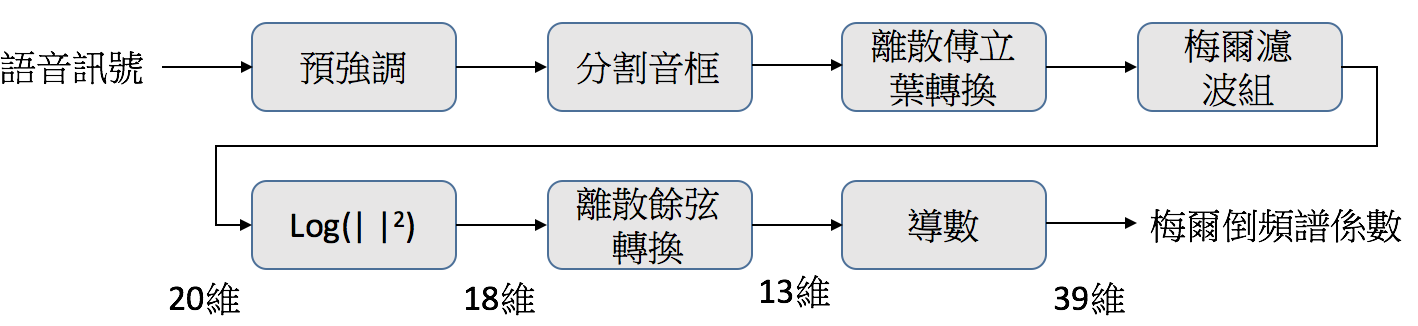
\includegraphics[scale=0.5]{images/ch3_mfcc.png} 
\caption{梅爾倒頻譜係數流程圖}
\label{ch3_mfcc}
\end{figure}

\begin{enumerate}
	\item 預強調

		語音訊號中高頻成分較低頻成分能量微弱許多,而語音的高頻成分蘊藏許多能辨別語音的資訊,因此將語音訊號做預強調,增加其高頻成分的比重,幫助語音訊號有較好的辨識效果。實作方法為將語音訊號通過一個高通濾波器
		(High-pass Filter),以提高其高頻成分的能量。
	\item 分割音框(Frame)
		
		語音訊號為時變訊號,其訊號特徵跟隨時間改變。為了分析語音訊號,將語音訊號分割成許多固定長度且彼此重疊的音框,並假設在音框內訊號特徵是穩定不變的。一般而言,音框的長度為20ms,而音框重疊的長度為10ms。且音框通常會乘上漢明窗 (Hamming Window) 以增加音框之間的連續性。
	\item 離散傅立葉轉換 (Discrete Fourier Transform, DFT)
		
		在時間軸進行分析並不容易,所以將語音訊號分割成音框後,對每個音框內的訊號進行離散傅立葉轉換,將每個音框內的時軸訊號轉為以頻率軸來表示。就訊號儲存的觀點來說,儲存完整的訊號是非常耗費資源的,且完整的訊號包含太多跟語音無關的資訊,其中只需要儲存有用的特徵即可。因此以下步驟大部份是為了壓縮訊號,提取關鍵訊號資訊為目的。
	\item 梅爾濾波組 (Mel-Filter Bank)
		
		梅爾濾波組由數組重疊的三角形濾波器所組成,如圖\ref{ch3_mel_filter}所示,其概念是模仿人類的聽覺神經。由於人類的聽覺神經對低頻部份較敏感,因此在低頻部份濾波器分佈較密集,高頻部分則較鬆散。取通過各濾波器的訊號能量做為參數。假設梅爾濾波組由20組三角濾波器組成,則經過濾波組後,每一個音框會被壓縮成一個20維的向量。再者,因為聽覺神經對音量的敏感度與訊號能量取對數成正比,為了模擬聽覺神經,我們對經過濾波組後得到的訊號能量取對數。

\begin{figure}[h]
\centering
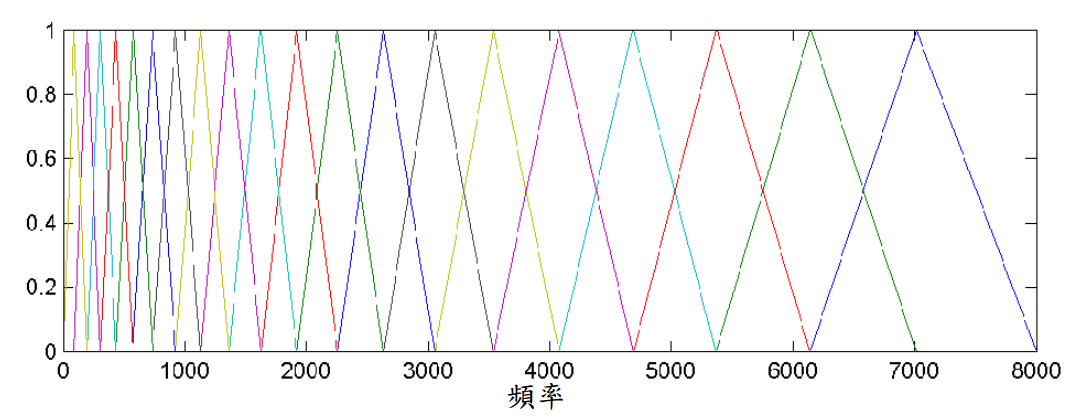
\includegraphics[scale=0.5]{images/ch3_mel_filter.png} 
\caption{梅爾濾波組}
\label{ch3_mel_filter}
\end{figure}
	\item 離散餘弦轉換 (Discrete Cosine Transform, DCT)
		
		梅爾濾波組是由彼此重疊的濾波器所組成,可以想像抽出來的參數其維度及維度之間有很大的相關性(Correlation)。為了進一步達到訊號壓縮的效果,將向量透過離散餘弦轉換,投射至維度彼此正交(Orthogonal)的軸上。忽略一些對訊號影響較小的維度後,此向量從20維降至12維,
		最後再將音框中總體訊號能量列入,每個音框以13維的向量來表示。由於離散餘弦訊號可以視為一種反離散傅立葉轉換
		(Inverse Discrete Fourier Transform,IDFT)
		,此步驟相當於將頻率軸的訊號又轉回類似時軸的空間中,而經過梅爾濾波組及取對數等的處理後,反離散傅立葉轉換後不能稱為時軸,學者便將其稱為倒頻譜
		(Cepstrum) ,即為梅爾倒頻譜係數名稱的由來。
	\item 取導數 (Derivatives)
		
		至離散餘弦轉換為止,梅爾倒頻譜係數只考慮音框內的訊號資訊,然而音框與音框之間的關係也蘊藏有許多語音的訊息。因此,我們對13維梅爾倒頻譜係數取一階及二階導數,並將其與本來的係數串接為39維的向量,其目的在於將音框之間的資訊也列入聲學特徵的考量中。
\end{enumerate}

產生出39維的梅爾倒頻譜係數後,接下來,使用倒頻譜平均數與變異數正規化法(Cepstral
Mean and Variance
Normalization,CMVN),將每一維度的參數平均值變為 $ 0 $ ,變異數變為 $ 1 $ ,如此能夠抵抗雜訊的干擾。數學式如\ref{CMVN}:

\begin{equation}
\begin{aligned}
X_{CMVN}[n] = \frac{ X[n] - \mu_x }{ \sigma_x } ,n = 1,2,...,N
\\
\\
\mu_{x} = \frac{1}{N} \sum_{n=1}^N {X[n]}, \sigma_x = \sqrt{\frac{1}{N}\sum_{n=1}^N{ (X[n] -\mu_{x} )^2}}
\end{aligned}
\label{CMVN}
\end{equation}
其中 $ X[n],n= 1, 2, ...,N $ ,為音框的倒頻譜係數,經過正規化的係數為 $ X_{CMVN}[n],n =
1,2,...,N $ , $ \mu_x $  為音框參數的平均數, $ \sigma_x $  為音框參數的標準差。

藉由上述的方法,可以將語音文件跟語音查詢詞,抽出其對應的聲學特徵。
\subsection{序列對序列模型(Sequence-to-Sequence Model)\cite{sutskever2014sequence}}
\begin{figure}[h]
\centering
\includegraphics[scale=0.5]{images/ch3_seq2seq.png} 
\caption{序列對序列模型}
\label{ch3_seq2seq}
\end{figure}
\label{seq2seq}
遞迴式類神經網路因其有記憶性,每個時間點的輸出,會依據之前記憶跟現在時間點的輸入改變。所以依照其特性,可以將語音文件一一給入模型中,在最後時間點的輸出,可以當做模型已經看過整個語音文件,產生的語音特徵向量。此想法跟序列對序列模型的概念相同,如圖~\ref{ch3_seq2seq}
所示。

序列對序列模型有兩個部分,分別為編碼器(Encoder)跟解碼器(Decoder),由兩個不同的遞迴類神經網路所組成,編碼器會先將輸入 $ X $ 依序讀過,跟先前的遞迴神經網路有點不同,會忽略編碼器的輸出,因為其目的是為了將輸入 $ X $ 依序看過轉變成為一個維度固定的隱藏狀態(Hidden
State)。解碼器則將編碼器的隱藏狀態當做初始,在每個時間點會依據隱藏狀態跟上個時間點的輸出產生出此時的輸出,產生解碼器此時的輸出,在最一開始的輸入,解碼器的輸入為零向量(Zero
Vector),如圖上的 $ 0 $ 。此種模型在機器翻譯(Machine
Translation)和自動摘要(Summarization)裡是很常見。在機器翻譯中,會先將欲翻譯的文字先經編碼器轉換成向量,再透過解碼器產生翻譯的文字。在自動摘要中,會將整篇文章先經過編碼器變成向量,利用解碼器輸出文章的摘要內容。

藉此可以將查詢詞跟語音文件藉由編碼器將原本為一連串的序列轉變成單一個隱藏狀態,再藉由最後一個時間點的輸出來代表文件或查詢詞的特徵向量表示,如圖\ref{ch3_RNNVC}。

\begin{figure}[h]
\centering
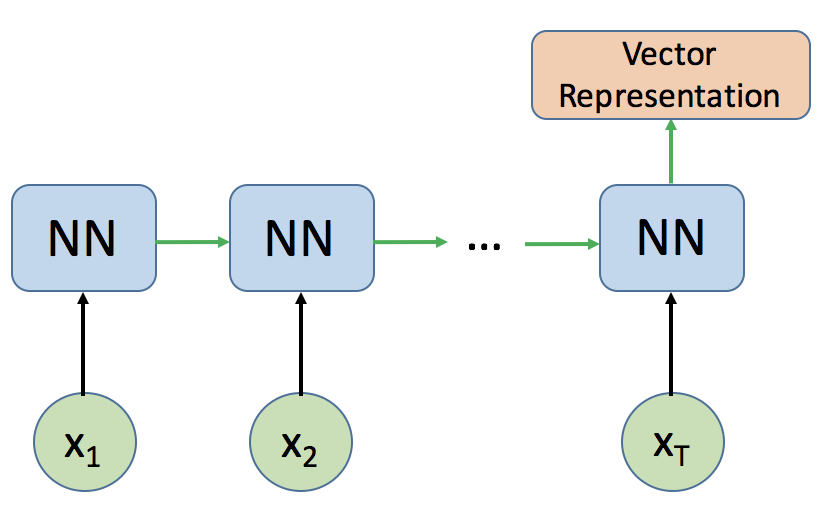
\includegraphics[scale=0.5]{images/ch3_RNNVC.png} 
\caption{遞迴類神經網路之向量表示}
\label{ch3_RNNVC}
\end{figure}

\section{系統架構}
\subsection{系統概觀}
\begin{figure}[h]
\centering
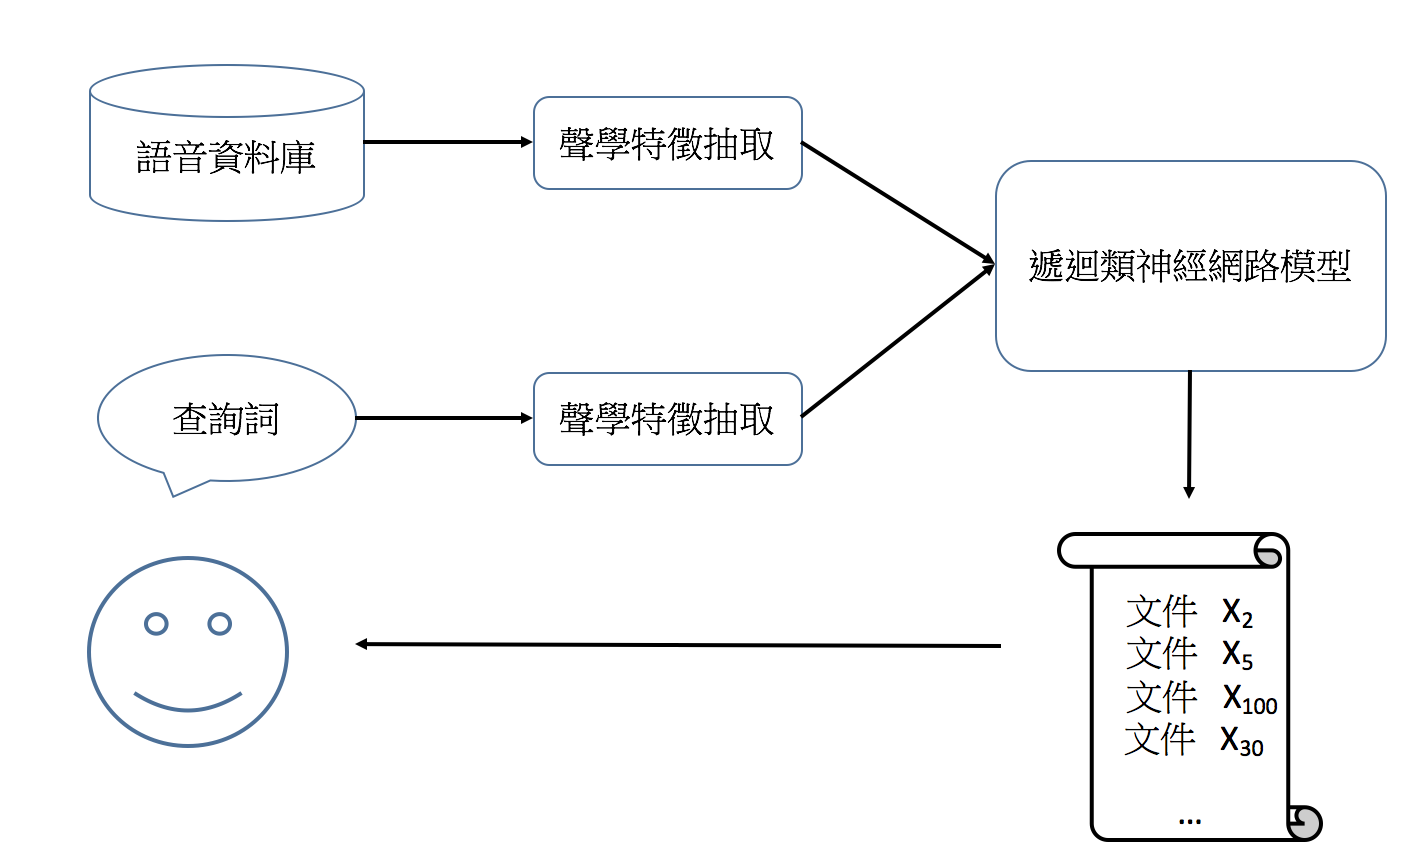
\includegraphics[scale=0.4]{images/ch3_system.png} 
\caption{系統概念圖}
\label{ch3_system}
\end{figure}
本章節所提出的口語詞彙架構如圖\ref{ch3_system}所示。主要為兩個部分,第一部分為特徵抽取,將查詢詞跟語音文件利用前述的方式進行聲學特徵抽取,抽取出 $ 39 $ 維梅爾倒頻譜係數。第二部分為遞迴類神經網路模型,將聲學特徵給入模型,最後模型會給予每個文件分數,來判定文件中是否出現查詢詞,此模型將在\ref{rnn_model}做介紹。
\subsection{遞迴類神經網路模型}
\label{rnn_model}
\begin{figure}[ht]
\centering
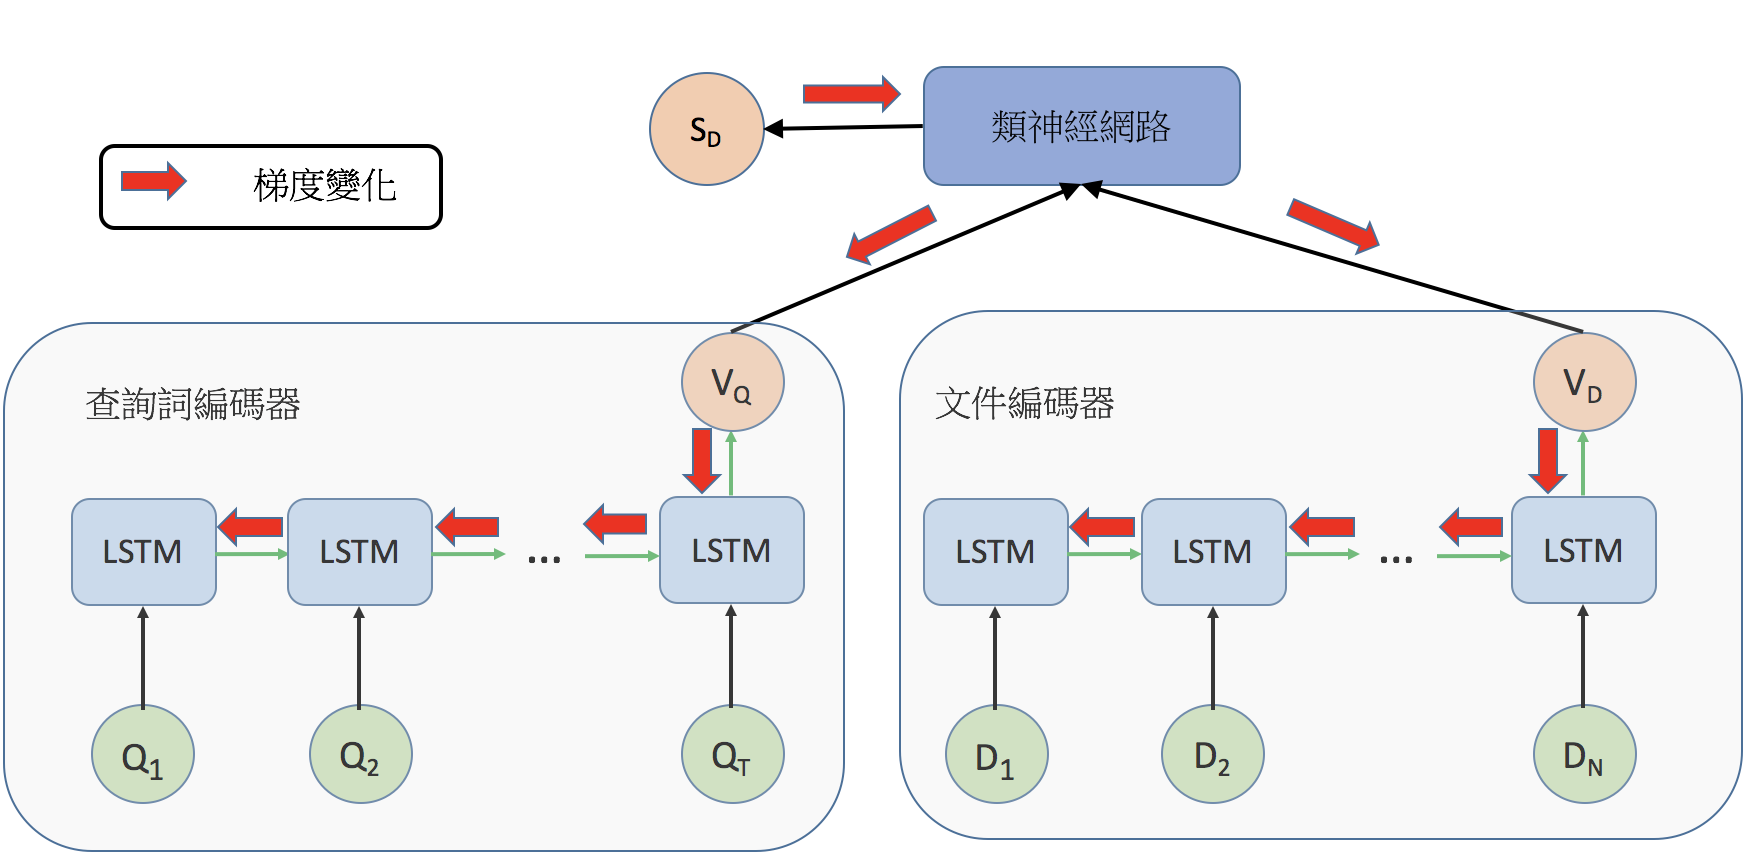
\includegraphics[scale=0.4]{images/ch3_RNN_model_g.png} 
\caption{遞迴類神經網路模型圖}
\label{ch3_RNN_model}
\end{figure}
圖\ref{ch3_RNN_model}為整個模型的架構圖,分為兩個部分,一個為遞迴類神經網路的編碼器,一個為類神經網路的分類器。編碼器負責將查詢詞跟語音文件分別由藉由它們的聲學特徵編碼成代表的向量特徵,類神經網路藉由向量特徵給予此文件一個分數。編碼器為前述\ref{LSTM}的長短期記憶網路(LSTM),且圖上的兩個編碼器參數是相同的。因此時口述詞彙偵測問題被視為分類問題,模型最後的輸出為兩維,一維代表查詢詞出現在文件當中的分數,一維則是未出現的分數,最後會在經過正規化,使兩維分數相加為 $ 1 $ 。

\subsection{訓練方式}
訓練類神經網路,需要先定義出損失函數。損失函數使用先前\ref{ch2_train_DNN}章提到交叉熵,來進行訓練。簡化的交叉熵為式子\ref{eq:ch3_LCE}
\begin{equation} 
\label{eq:ch3_LCE}
L_{CE}(\bold{x} , \bold{y} , \theta) = KL( \bold{y} ||\hat{\bold {y}} )  = - \log \hat{y}_{l} 
\end{equation}
其中KL為克雷散度, $ \hat{y}_{l} $ 為模型給正確標籤的分數。在最小化損失函數的同時,也就將正確標籤的分數提高,使模型能夠分類越準確。整個模型的訓練採用端對端訓練(End-to-End
Training),亦即不需要獨立訓練編碼器的部分,直接由輸出端的梯度變化,向後傳遞藉此訓練編碼器,如圖\ref{ch3_RNN_model}紅色箭頭所表示,則不須費心在編碼器產生的向量品質好壞,完全交由模型自動訓練跟判斷。
\section{實驗結果與分析}
\subsection{實驗設定}
 實驗語料採用LIBRISPEECH~\cite{panayotov2015librispeech}的英文語料,這是使用LibriVox的應用程式介面(LibriVox's
 API)收集參加讀者的閱讀訊息、音頻及閱讀書籍的章節。語料庫的內容大小不同,利用華爾街日報(The
 Wall Street Journal,
 WSJ)~\cite{paul1992design}語料庫裡的Si-84當作訓練語料,訓練出語音辨識模型,根據此模型測試的詞錯誤率(Word
 Error
 Rate,WER)大約分成三個子集合,分別為100小時、360小時與500小時。前兩組語料為詞錯誤率較小的集合,故以clean稱之,其中每位講者時間限制為25分鐘以避免權重不平衡,此兩個語料集合口音較接近美式英語,而最後500小時為詞錯誤率較高則以other稱之。表\ref{table:ex_info}提供了Librispeech的集合資訊。
 \begin{table}[ht]
	 \caption{Librispeech 集合列表}
	 \label{table:ex_info}
 \begin{tabular}[t]{|l|l|l|l|l|l|}
	 \hline
	 集合 & 時間(hr) & 講者時數(min) &女性講者人數&男性講者人數&總講者\\
	 \hline
	 train-clean-100   & 100.6   & 25 & 125 & 126 & 251 \\
	 \hline
	 train-clean-360   & 363.6   & 25 & 439 & 482 & 921 \\
	 \hline
	 train-other-500   & 496.7   & 30 & 564 & 602 & 1166 \\
	 \hline
 \end{tabular}
 \end{table}
 
 本篇論文將train-clean-360 當作訓練語料,將train-other-500
 當作測試語料。利用TF-IDF(Term Frequency–inverse Document
 Frequency)分別對訓練和測試語料做排序,訓練語料中選出500個查詢詞,70,000筆的訓練資料,測試語料30個查詢詞,1,000筆測試資料。且限制語音文件的長度為15秒,語音查詢詞的長度為2秒。
\subsection{基準實驗}
本章所使用的基準實驗為前述\ref{sec:chap4_sdtw}章所提到的片段式動態時間校準,利用動態時間校準可以計算出查詢詞聲學特徵跟語音文件聲學特徵的最相關的距離。依照此距離來將文件進行排序,計算平均準確率。基準實驗在測試語料上獲得的平均準確度為 $ 0.6173 $ 。
\subsection{實驗結果與分析}
 \begin{table}[ht]
	 \centering
	 \caption{遞迴類神經網路實驗結果}

	 \label{table:ch3_exp}
	 \begin{tabular}{|c|c|c|}
		 \hline
		 \multicolumn{2}{|c|}{模型架構} & 平均準確率 \\
		 \hline
		 \multicolumn{2}{|c|}{基準實驗} & 0.6173 \\
		 \hline
		 \hline 
		 編碼器 & 類神經網路結構 & 平均準確率  \\
		 \hline
		 \multirow{3}{*}{兩層LSTM} & 128-2 & 0.5753\\
		 \cline{2-3}
		 & 128-64-32-2 & 0.5935 \\
		 \cline{2-3}
		 & 128-128-128-2 & 0.6076\\
		 \hline
		 \multirow{2}{*}{三層LSTM} & 128-64-32-2 & 0.5950 \\
		 \cline{2-3}
		 & 128-128-128-2 & 0.6025 \\
		 \hline
		 \multirow{2}{*}{兩層GRU} & 128-64-32-2  &  0.6080\\
		 \cline{2-3}
		 & 128-128-128-2 & 0.6070 \\
		 \hline
		 \multirow{2}{*}{三層GRU} & 128-64-32-2  & 0.6010 \\
		 \cline{2-3}
		 & 128-128-128-2 & 0.5965 \\
		 \hline
	   \end{tabular}
 \end{table}

表\ref{table:ch3_exp}為本章的實驗結果,比較了各模型與基準實驗的表現,使用平均準確率來做衡量標準。在本章的編碼器採用了兩種遞迴類神經細胞,一種為\ref{LSTM}章介紹的長短期記憶細胞(LSTM),另一種記憶細胞為門閘遞迴單元(Gated
Recurrent Unit,
GRU)~\cite{cho2014learning},是長短期記憶細胞的簡化版。輸入門限和遺忘門限是連動的,當遺忘門限關閉清除儲存內容時,輸入門限才會開啟儲存新的資料。編碼器的記憶細胞數量為128,也就是語音文件跟查詢詞經由編碼器產生出128維度的向量表示。類神經網路分類器的部分採用了各種結構如表\ref{table:ch3_exp}上所示,以128-64-32-2
來說,類神經網路的架構即為第一層128個類神經元,第二層64個,第三層32個,最後一層為2個。模型的學習率皆為0.001,並使用二次正規化來避免模型過度貼合。

從表中可以看出類神經網路128-2的表現,相比於其他128-128-128-2、128-64-32-2結構,少了2\%的平均準確率,因深層的模型可以有效提高分類正確率。對於不同類型的遞迴神經網路GRU跟LSTM的表現是差不多的,且模型的層數也對平均準確率影響不大。綜觀所有模型,平均準確率大約落在0.6,仍無法贏過基準實驗的0.6173。因模型僅僅簡單的將語音文件轉化成一個向量,可能無法充分表示此語音文件,語音文件不只有一個詞而是一整段句子,語音文件向量會遺失掉某些詞的資訊。即使分類器在強大,仍無法準確檢索出來。
\\
\\
\\

\section{本章總結}
本章使用了遞迴類神經網路來產生出語音文件跟查詢詞的單一特徵向量表示,由於遞迴類神經網路有著序列順序前後關係及空間的不變性,可以有效的將序列的語音文件,描述成單一向量表示。產生代表語音文件跟查詢詞的向量表示後,再藉由多層類神經網路分類器依據向量表示來判斷查詢詞出現與否。本章提出了一個基本的檢索模型,無須經過語音辨識系統,能夠直接在聲學特徵上進行檢索。雖其表現都輸給基準實驗一小段差距,不過平均準確率也大致能夠達到0.6,顯示出利用遞迴類神經網路做檢索是可行的,並非完全失敗,之後將以此模型為雛形進行改良。
